\section{Mini}
\begin{frame}
\begin{center}
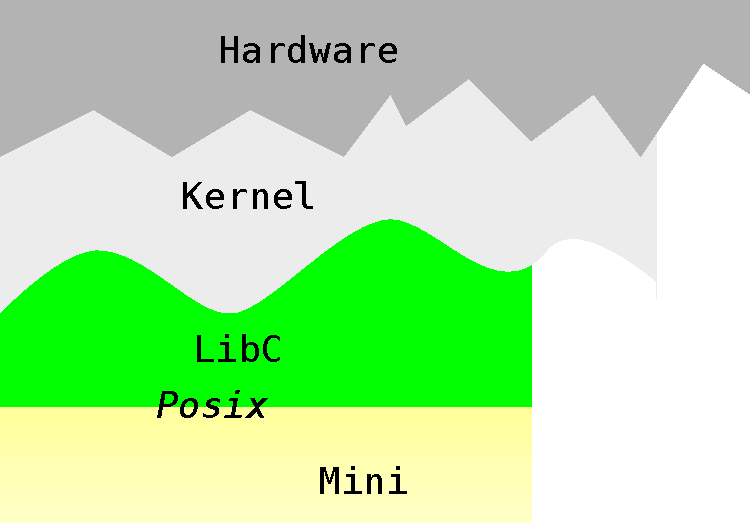
\includegraphics[width=0.5\textwidth]{mini.pdf}
\end{center}
\vspace{-5mm}
\begin{itemize}
 \item \cod{config/Makefile}
 \item \cod{src/cc-mini.cc}
 \begin{itemize}
  \item static
  \begin{description}
   \item[target-root] \cod{libc.a}
  \end{description}
  \item dynamic
  \begin{description}
   \item[target-root] \cod{libc.so}, \cod{loader}
  \end{description}
 \end{itemize}
\end{itemize}
\end{frame}

\subsection{Libraries}

\begin{frame}{Statische/Dynamische Bibliothek}{Kopie vs. Referenz}
 \begin{columns}
  \begin{column}{5cm}
   \begin{block}{Static}
   \begin{itemize}
    \item \hfill \vspace{-3mm}\fig{static.pdf}{0.5}{0}
    \item {\Large frühes} Binden
   \end{itemize}
   \end{block}
  \end{column}
  \begin{column}{5cm}
   \begin{block}{Dynamic}
    \begin{itemize}
    \item\hfill \vspace{-3mm}\fig{dynamic.pdf}{0.5}{0}
    \item {\Large spätes} Binden
    \end{itemize}
   \end{block}
  \end{column}
 \end{columns}
 \begin{block}{}
  \fig{legend.pdf}{0.5}{0}
 \end{block}
\end{frame}

\begin{frame}{Dynamische Bibliothek:der Loader}{am Beispiel \cod{mini.c}}
 \begin{itemize}
  \item wir sind in \cod{work}
  \item \cod{gcc ../src/mini.c -o mini} 
  \item \cod{file mini}
  \item start loader
  \item start loader mit {\em executable}
 \end{itemize}
\end{frame}

